%======================================================================
\chapter{Introduction}
%======================================================================

%----------------------------------------------------------------------
\section{Background}
%----------------------------------------------------------------------
Japan has long been one of the most popular tourist destinations in Asia. Before the spread of Covid-19, the number of foreign visitors to Japan gradually increased. According to Japan National Tourism Organization (JNTO) statistics, the number of foreign visitors more than quadrupled between 2012 (8.36 million) and 2019 (31.9 million) that shown in Figure~\ref{fig1}. As a result, the Japan National Tourism Organization has been working hard over the years to assist foreign visitors to have a better experience in Japan. Considering that Japan is a relatively disaster-prone country, disaster prevention for foreign visitors during their stay in Japan has been an issue of great concern to the Japan National Tourism Organization.

%%%%%%%%%%%%%%%%%%%%%
%\iffalse
\begin{figure*}[h]
  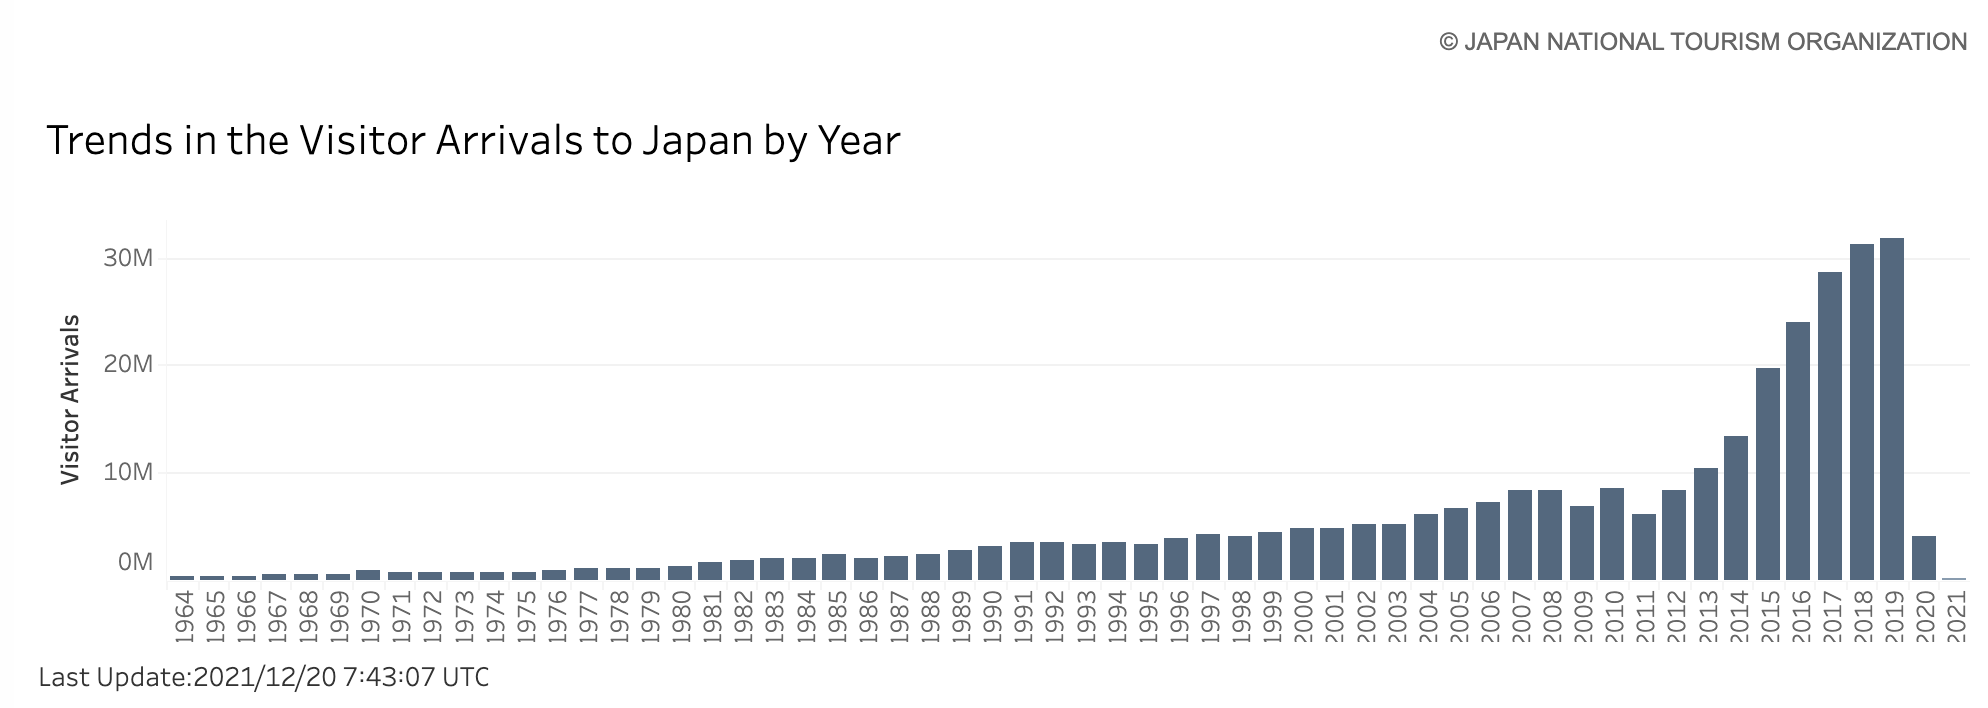
\includegraphics[width=\linewidth]{Figure/Figure1.png}
  \centering
  \caption[Foreign visitors number in Japan by year.]{Foreign visitors number in Japan by year.\protect\footnotemark }
  \label{fig1}
\end{figure*}
\footnotetext{https://statistics.jnto.go.jp/en/graph/\#graph--inbound--travelers--transition}
%\fi

After the 2018 Hokkaido Eastern Iburi earthquake, Survey Research Center, Inc. conducted a survey~\footnote{https://www.surece.co.jp/wp\_surece/wp-content/uploads/2018/09/20180914\_Result.pdf} on the evacuation behavior of foreign visitors to Japan. Survey Research Center, Inc. completed this survey in collaboration with JTB Corporation. The survey was completed on September 8th (Saturday) and 9th (Sunday), 2018. The survey chose the Hokkaido Tourism Information Center on Tanukikoji Shopping Street as the survey spot, and interviews were conducted by foreign-language speaking surveyors using the survey questionnaire. The survey collected 185 valid samples from foreign tourists visiting Japan who stayed in Hokkaido on September 6, 2018, asking about their behavior during the earthquake, evacuation guidance provided by accommodation facilities, and problems encountered during the earthquake. Mainland China, Taiwan, Hong Kong, the United States, and South Korea accounted for 70\% of the respondents' nationalities. The study's findings reveal a number of significant findings, including difficulties in earthquakes, behaviors have taken after the disaster happened, and desired response in the event of an earthquake.

First, the survey result of difficulties encountered by foreign visitors during the earthquake was shown in Figure~\ref{fig2a}. The inability to access information due to power outages and the inability to charge cell phones were the top-ranked difficulties. The third most difficult problem was a lack of supplies in supermarkets and convenience stores. The fourth-ranked difficulty was the schedule change caused by the earthquake. The fifth concern was not knowing where to go or what to do because of a language barrier. Lack of food/water supplies, uncertainty about the next trip, inability to understand earthquake information shown on TV, lack of information provided by transportation agencies/airports, and lack of earthquake evacuation manuals for foreigners that make it difficult to know what to do were the sixth to tenth-ranked difficulties. The lack of multilingual disaster/transportation/evacuation information in cell phones, the lack of evacuation instructions in hotels, the lack of information about the earthquake in Japan, the lack of information about what to bring to evacuate, and the lack of information from medical institutions were the eleventh to fifteenth difficulties. According to the results, the most common difficulties during the earthquake, were related to power outages, such as 'power outages made it difficult to get information' and 'power outages made it difficult to charge smartphones, etc' ( 67.0\%). Due to unforeseen circumstances caused by the earthquake, the response of 'lack of supplies at convenience stores and supermarkets'  (46.5\%) was also common. Respondents were concerned about modifications to their itinerary as a result of transportation disruptions, such as 'all my itineraries were disrupted and I had to pay a lot of money' (37.3\%) and 'I couldn't predict what would happen to my itinerary in the future'(27.0\%). Another common difficulty was related to language issues like 'I didn't know where to go because I didn't understand the language' (29.2\%).

Second, Figure~\ref{fig2b} shows the survey results of behaviors that occurred after the earthquake. Following the earthquake, the top three common actions were 'tried to get information via the Internet or SNS' (49.7\%), 'stayed where they were and checked on the situation' (44.3\%), and 'kept in touch with family and friends via the Internet, e-mail, and SNS such as Facebook and Line' (39.5\%). Calling family/friends (31.9\%), getting information about the earthquake from TV or radio (31.4\%), contacting the hotel front desk (27\%), and contacting fellow travelers (20\%) was the fourth to seventh popular responses. So, based on the survey results, we can conclude that after the earthquake, people prefer to stay in the area to look into the matter while gathering information and confirming their safety via the Internet and social media. In particular, we can discover that there are two main ways for respondents to gather information. The first is face-to-face information-seeking behaviors, such as asking people around, hotel staff, and so on. The other type of information-seeking behavior is no-face-to-face information-seeking behaviors. The other is no-face-to-face information-seeking behaviors, which primarily rely on television/radio/social media/internet. We will also divide people's information-seeking behaviors into these two types in the follow-up study to see whether people's behavioral patterns are more inclined to contact people or not.

%%%%%%%%%%%%%%%%%%%%%%%%%%%%%%%%
%\iffalse
\begin{figure*}[h]
  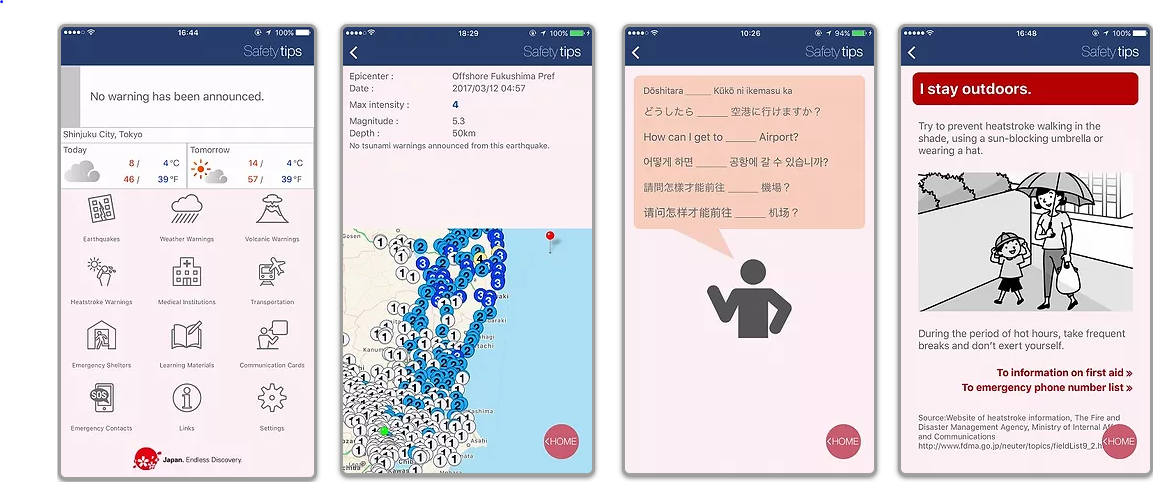
\includegraphics[width=\linewidth]{Figure/Figure3.png}
  \centering
  \caption[Safety Tips' interface]{Safety Tips' interface.\protect\footnotemark }
  \label{fig3}
\end{figure*}
\footnotetext{https://www.rcsc.co.jp/safety}

\begin{figure*}[h]
  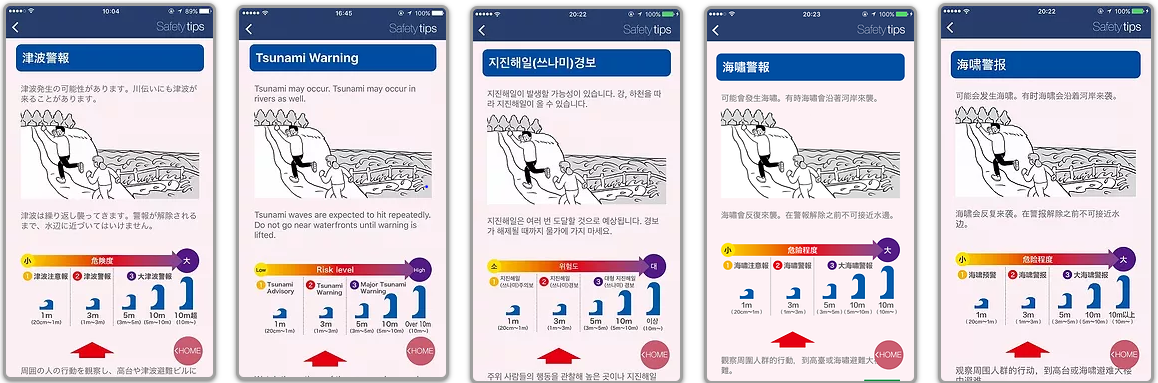
\includegraphics[width=\linewidth]{Figure/Figure4.png}
  \centering
  \caption[Multilingual Notifications for Safety Tips]{Multilingual Notifications for Safety Tips\protect\footnotemark }
  \label{fig4}
\end{figure*}
\footnotetext{https://www.rcsc.co.jp/safety}
%\fi

Third, as shown in Figure~\ref{fig2c}, popular desired responses in the event of an earthquake were 'Provide charging points, etc.' (50.8\%) and 'Enhance information centers' (42.2\%), followed by 'Distribute manuals in native languages' (38.4\%). And the next most common responses can be roughly divided into three categories. The first is a requirement for multilingual services, such as 'want evacuation guidance in a language I understand' (36.2\%) or 'want disaster/traffic/evacuation information to be provided in multiple languages via smart phones, etc.' (35.1\%), 'Would like TVs and other media to display information in English' (30.8\%), 'Would like information signs in my native language' (24.9\%). Another requirement was for a place of evacuation, such as 'providing places to stay and other accommodations'(34.6\%), 'Would like the hotel where I was staying to serve as a disaster information hub' (22.2\%). The last category was for providing information, such as 'Would like information centers to be set up to provide information on transportation and flights' (25.4\%), 'Provide telephone consultation services'(15.1\%), and 'Would like pamphlets and other materials that show what to do after an evacuation'(14.1\%), and 'Wish to learn more about medical institutions' (9.2\%).

Combined with the previous findings in the survey, it is clear that there is a need to provide sufficient places for foreign visitors to recharge in order to ensure that they can contact their family/friends and gather the necessary disaster information from social media/networks. The following step is to provide information in their language as well as evacuation assistance.

Considering the Japan Tourism Agency has constantly concern with issues of security and safety in the tourism industry. So, under the supervision of the Japan Tourism Agency, R.C. Solutions, Inc. developed a free application called Safety tips, which can notify foreign visitors of earthquake early warnings, tsunami warnings, eruption alerts, special warnings, heatstroke information, national protection information, evacuation advisories, and other disasters that occurred in Japan. Figure~\ref{fig3} shows the Safety Tips interface. During disasters, safety tips can provide a variety of purposes for foreign visitors to Japan. It is available in 14 languages (15 languages), including Japanese, English, Chinese (traditional and simplified), Korean, Spanish, Portuguese, Vietnamese, Thai, Indonesian, Tagalog, Nepali, Khmer, Burmese, and Mongolian (as shown in Figure~\ref{fig4}). Safety Tips is an important part of this study. The study will compare the difference in attitudes toward Safety Tips among respondents of various nationalities, as well as the differences in attitudes toward Safety Tips among people from various upbringing backgrounds.

%%%%%%%%%%%%%%%%%%%%%%%%%%%%
%\iffalse
\begin{figure*}[h]
  \begin{subfigure}{\textwidth}
    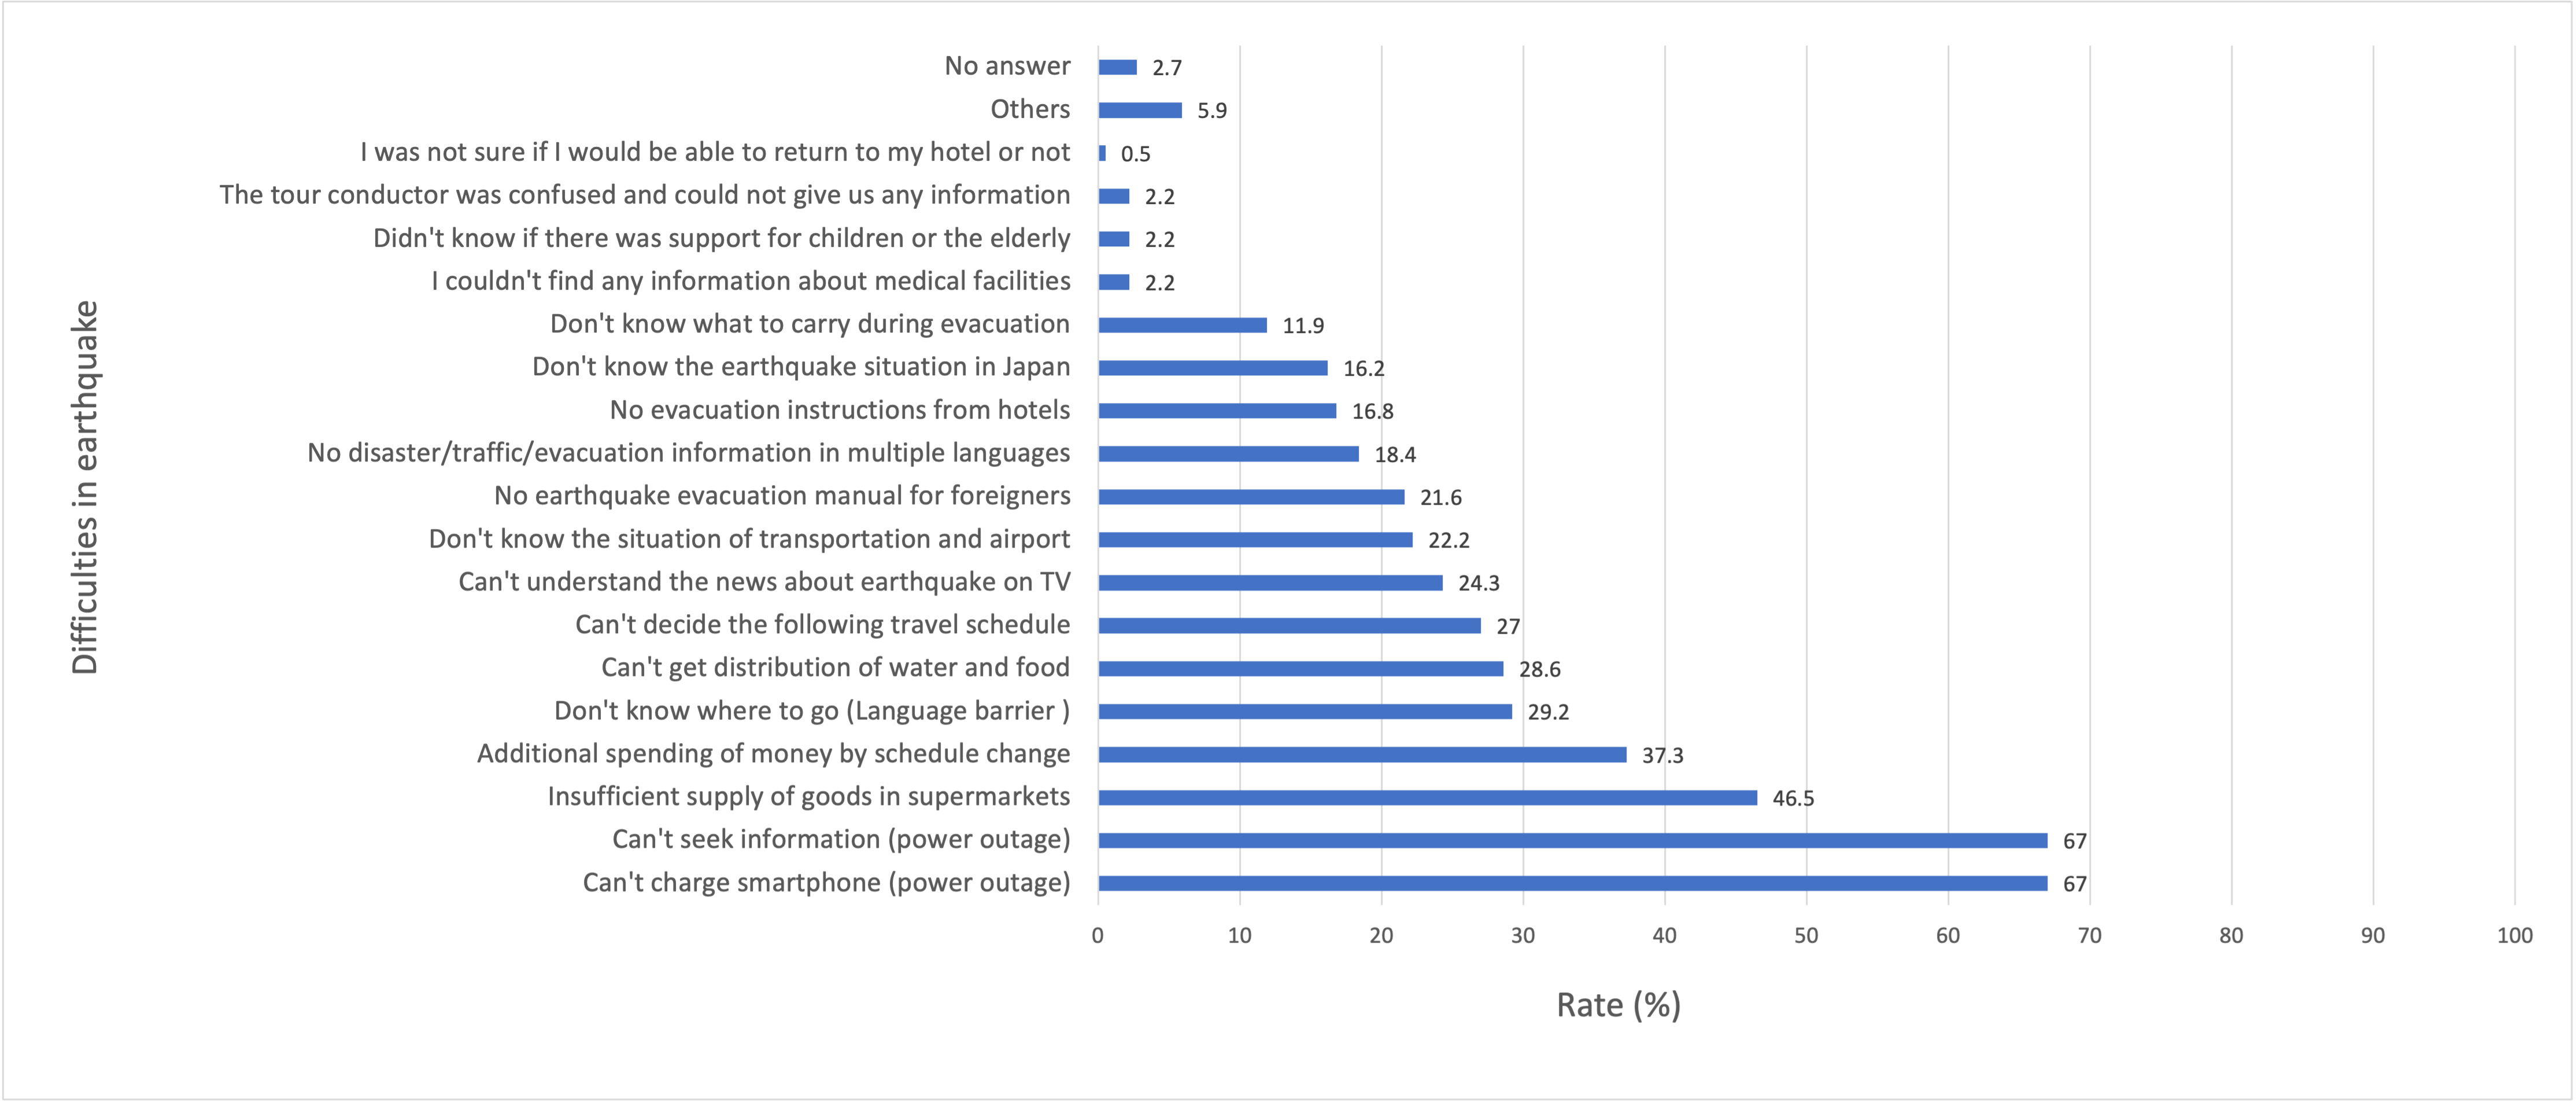
\includegraphics[width=\linewidth]{Figure/Figure2a.png}
    \caption{Difficulties in earthquake}
    \label{fig2a}
  \end{subfigure}
  \begin{subfigure}{\textwidth}
    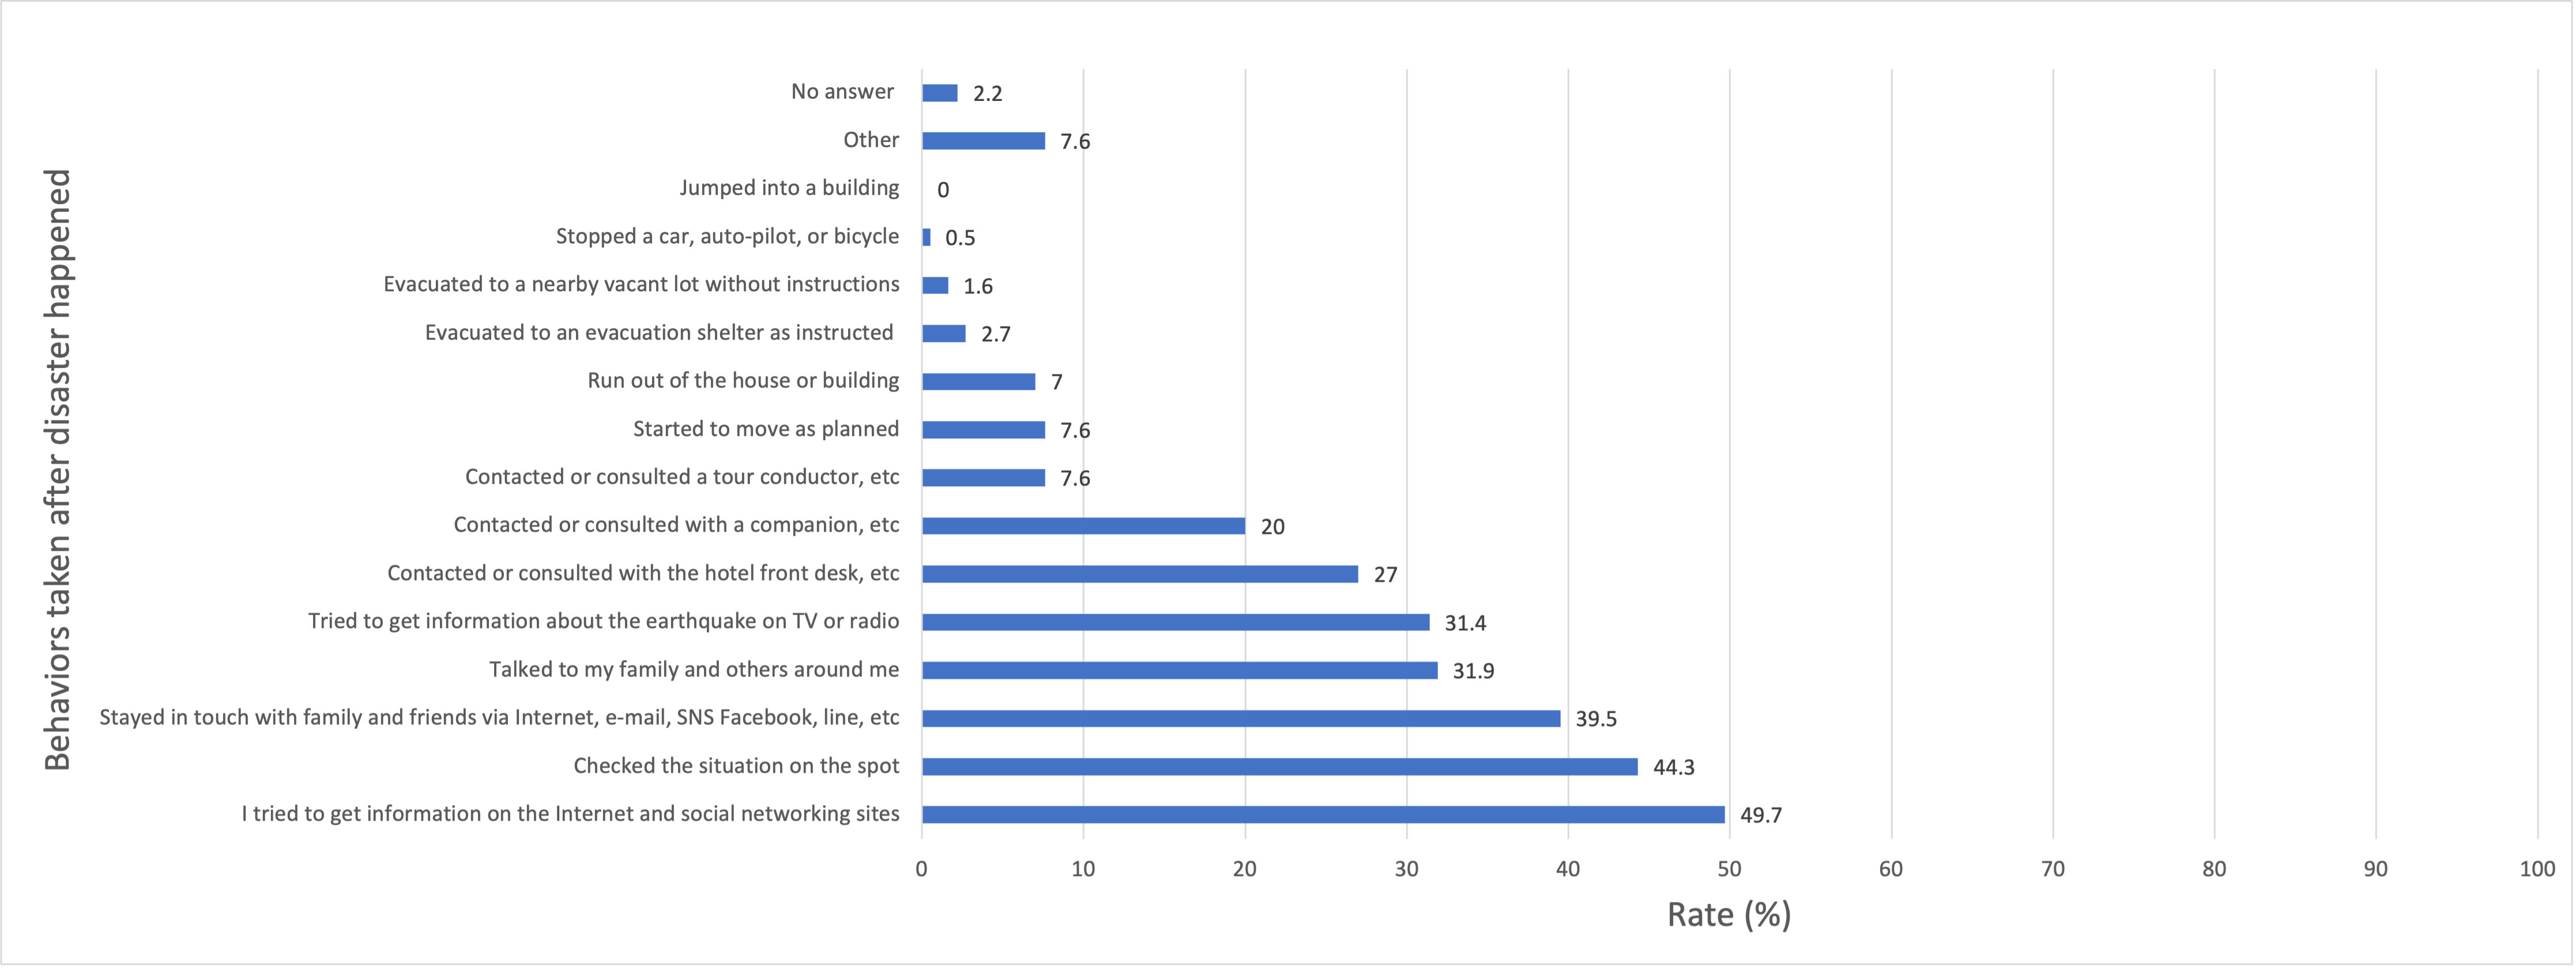
\includegraphics[width=\linewidth]{Figure/Figure2b.png}
    \caption{Behaviors taken after the disaster happened}
    \label{fig2b}
  \end{subfigure}
  \begin{subfigure}{\textwidth}
    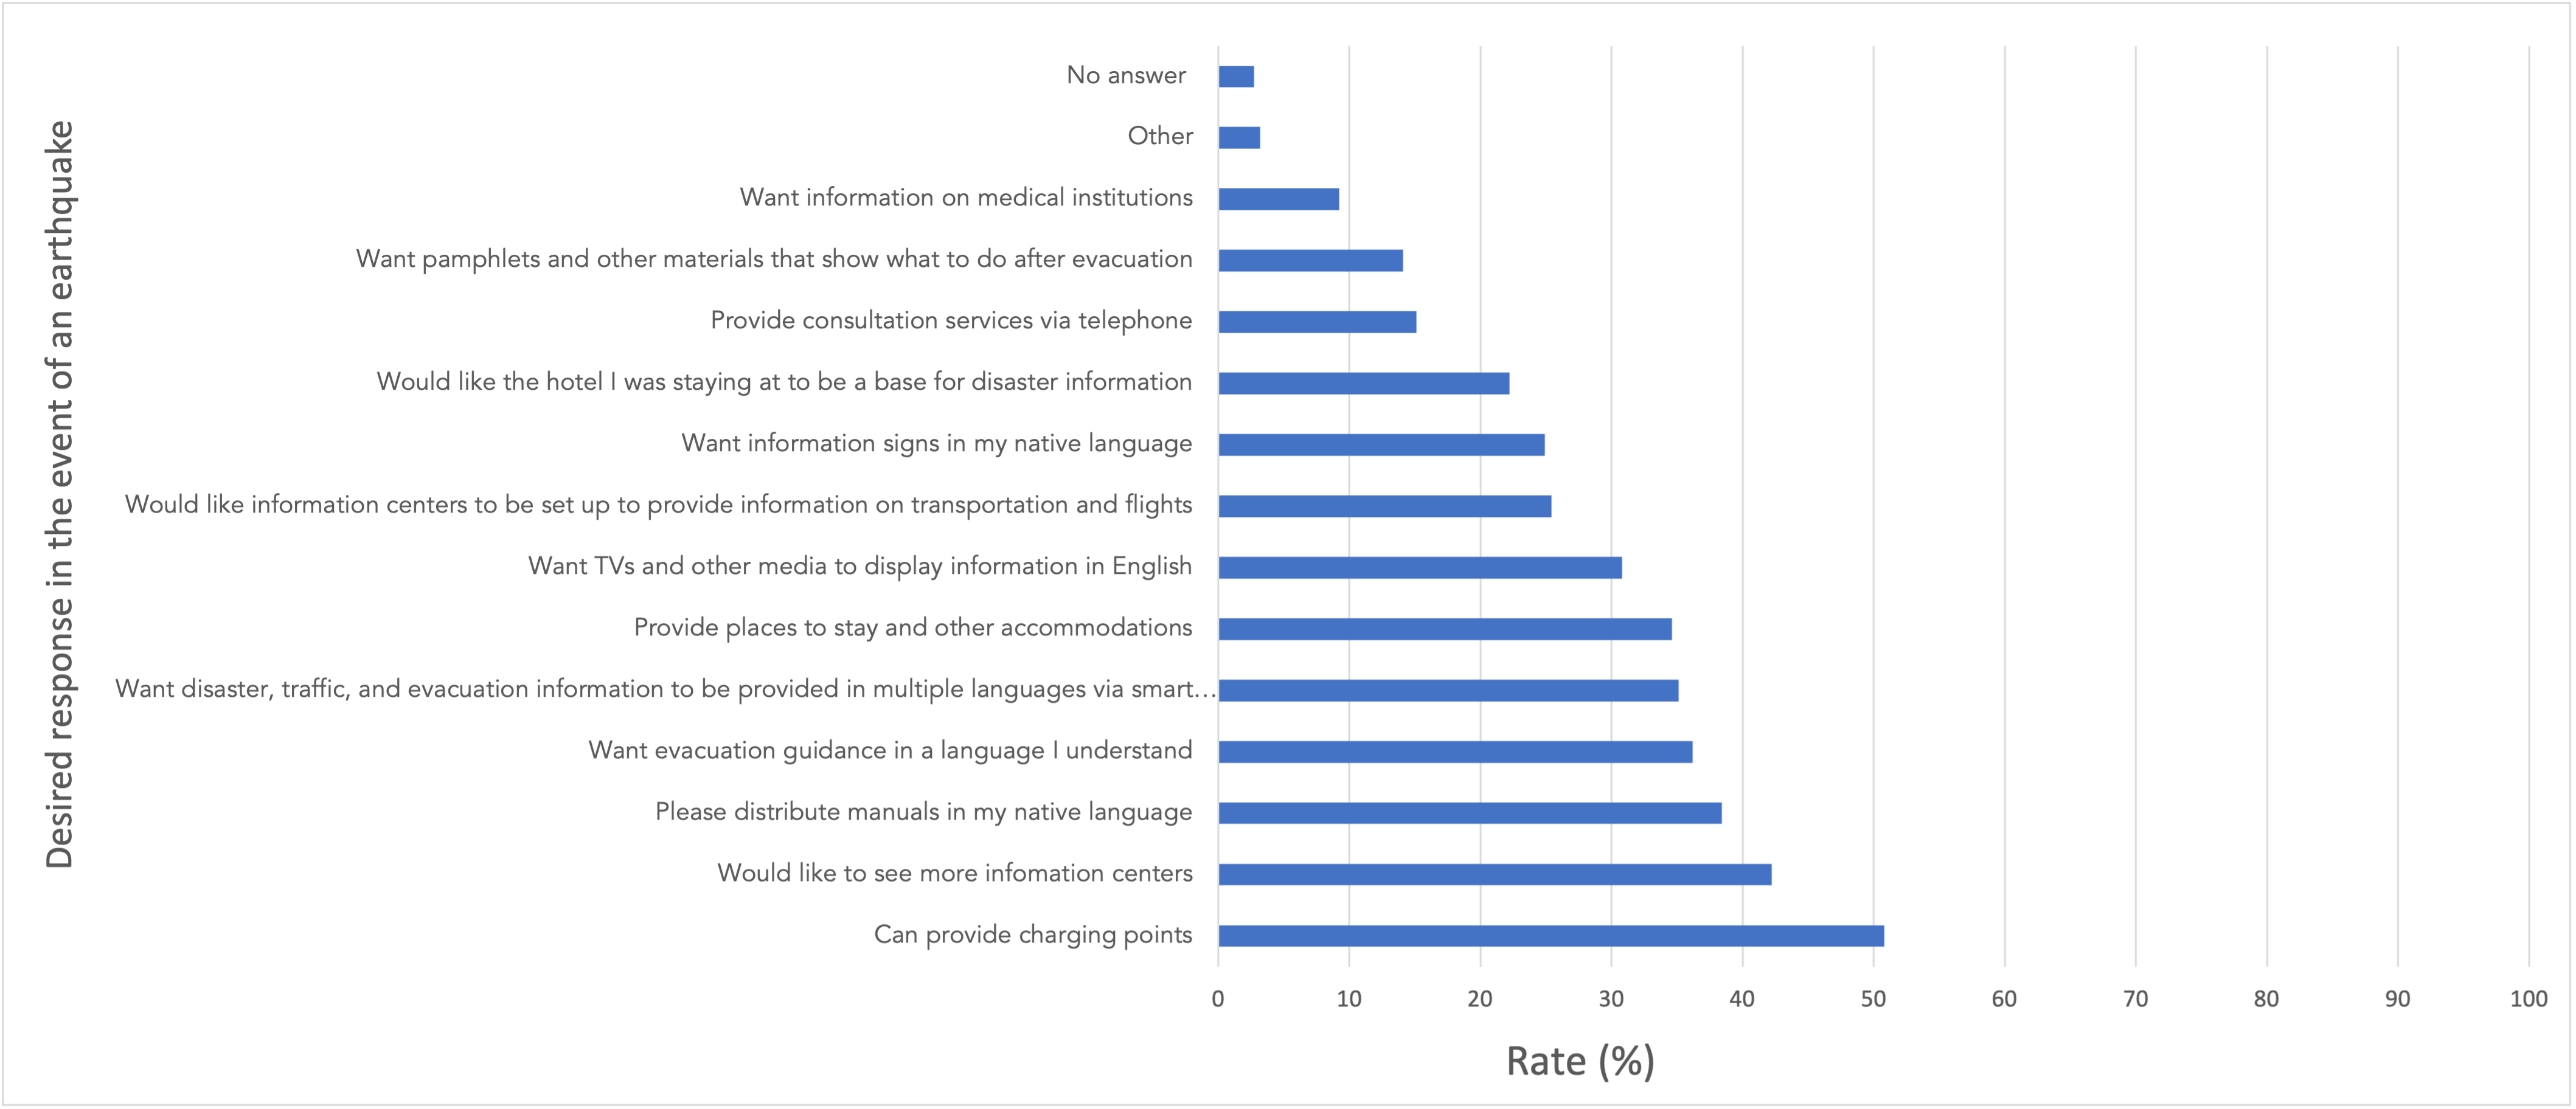
\includegraphics[width=\linewidth]{Figure/Figure2c.png}
    \caption{Desired response in the event of an earthquake}
    \label{fig2c}
  \end{subfigure}
  \centering
  \caption[Survey on Evacuation Behavior of foreign visitors to Japan after the 2018 Hokkaido Eastern Iburi earthquake.]{Survey on Evacuation Behavior of foreign visitors to Japan after the 2018 Hokkaido Eastern Iburi earthquake.\protect\footnotemark }
  \label{fig2}
\end{figure*}
\footnotetext{https://www.surece.co.jp/research/2491/}
%\fi
\cleardoublepage

\section{Problem Identification}
Based on the above, we can understand that foreign visitors will face numerous challenges when a disaster strikes while visiting. Because earthquakes and other natural disasters are relatively common in Japan, Japanese children learn about evacuation at a young age and participate in numerous evacuation/evacuation drills and exercises. However, there would be many differences between Japanese and foreign visitors. For example, for foreign visitors, it is unknown whether they have previously experienced disasters, whether they learned about evacuation as children, or whether they have participated in earthquake simulation drills. As a result, they would behave differently with the Japanese during the evacuation. Therefore, it is important to explore the behavioral differences between foreign visitors and Japanese. The results of a questionnaire survey were analyzed in this study to explore the patterns of evacuation behavior preferred by foreign visitors, as well as the differences between Japanese and foreign visitors.

Furthermore, to make Safety Tips more useful to foreign visitors, we first should understand their attitudes toward the use of Safety Tips. As a result, the first section of this study will explore the difference in attitudes toward Safety Tips among foreign visitors from various countries. Second, we will explore whether their prior use of Safety Tips influences their subsequent attitudes toward Safety Tips. In addition, structural equation modeling will be used in this order to examine how some personal characteristics influence respondents' attitudes toward Safety Tips. The personal characteristics include nationality, age, travel experience, disaster prevention education level, language ability, disaster experience, disaster prevention consciousness. These are discussed in depth in Chapter~\ref{c3}.

\section{Research Goal and Objective}
The goal of this study is to clarify the information-seeking and evacuation behavior of foreign visitors to Japan, as well as their perception of Safety Tips. 

This study has three main research objectives. The first objective is to understand foreign visitors' attitudes toward Safety Tips. The second objective is to explore how respondents' attitudes toward Safety Tips are influenced by their characteristics. The third objective is to explore the patterns of information seeking and evacuation behaviors, including which behavior comes first after the disaster happens and which behavior was used more frequently during the disaster. Finally, based on the findings of the research, provide improvement suggestions to Safety Tips.


\section{Thesis Structure}
This thesis begins with the first chapter, introduction, which explains the study's background, research questions, objectives and goals, and thesis structure. The introduction chapter's purpose is to provide background for the entire study and to help the reader in understanding the research topic. Then, the second chapter of the thesis focuses on the literature review. Considering that in this study, it is necessary to make the basic hypothesizes of Structural Equation Modeling based on prior research, so Chapter~\ref{c2} reviews some relevant studies in the field of evacuation research and establishes the basic hypothesizes of relationships between factors like demographic information, educational background, past disaster experience, and disaster training experience. The interpretation of the survey and data used in this study are presented in Chapter~\ref{c3}. Because the data in this study is extensive and complex, I intend to provide a more complete description in Chapter~\ref{c3} to help the reader understand it better. Chapter~\ref{c4} is about methodology, which includes the introduction and academic explanation of each methodology used to achieve each of the research objectives. Next, Chapter~\ref{c5} is results and analysis. Since this research is based on the analysis of data to clarify foreign visitors' behaviors and make suggestions of Safety Tips, this chapter shows and analyzes the results of the model one by one. The final chapter, Chapter~\ref{c6}, is the conclusion section. This chapter contains a summary conclusion of the whole study, some suggestions based on the results to help Safety Tips for better development, and the limitations in this study.

